\documentclass[tikz,border=10pt]{standalone}
\begin{document}
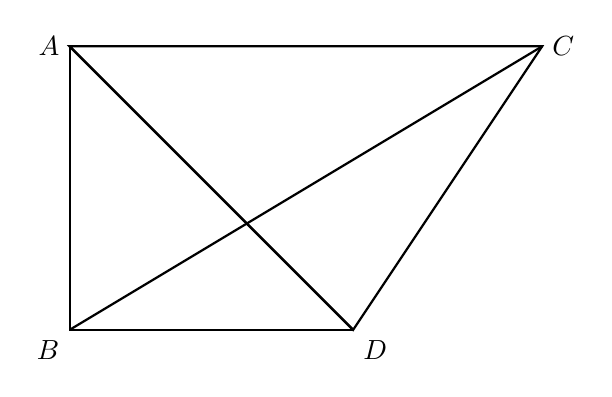
\begin{tikzpicture}[thick, scale=1.2]
    % 1. 定义坐标点
    \coordinate (B) at (0,0);
    \coordinate (A) at (0,3);
    \coordinate (D) at (3,0);
    \coordinate (C) at (5,3);

    % 2. 绘制多边形边框
    \draw (A) -- (C) -- (D) -- cycle; % 外部轮廓
    \draw (A) -- (B) -- (D);           % 左侧与底部边界
    \draw (B) -- (C);                 % 对角线 BC
    \draw (A) -- (D);                 % 对角线 AD

    % 3. 标注顶点标签
    \node[left] at (A) {$A$};
    \node[below left] at (B) {$B$};
    \node[right] at (C) {$C$};
    \node[below right] at (D) {$D$};

    % 4. 可选：若需标注直角符号
    % \draw (0.2,0) -- (0.2,0.2) -- (0,0.2); 
\end{tikzpicture}
\end{document}